\documentclass{article}
\usepackage[margin=1in]{geometry}
\usepackage{amsmath,amsthm,amssymb}
\usepackage{bbm,enumerate,mathtools}
\usepackage{tikz,pgfplots}
\usepackage{chessboard}
\usepackage[hidelinks]{hyperref}
\usepackage{multicol} % Problem 35
\usepackage{xstring} % Difficulty command
\usetikzlibrary{shapes.geometric}

\newenvironment{question}{\begin{trivlist}\item[\textbf{Question.}]}{\end{trivlist}}
\newenvironment{note}{\begin{trivlist}\item[\textbf{Note.}]}{\end{trivlist}}
\newenvironment{references}{\begin{trivlist}\item[\textbf{References.}]}{\end{trivlist}}
\newenvironment{related}{\begin{trivlist}\item[\textbf{Related.}]\end{trivlist}\begin{enumerate}}{\end{enumerate}}

\newcommand\score[1]{
\pgfmathsetmacro\pgfxa{#1+1}
\tikzstyle{scorestars}=[
  star,
  star points=5,
  star point ratio=2.25,
  draw,
  inner sep=3pt,
  anchor=outer point 5
]
  \begin{tikzpicture}[baseline]
    \draw[opacity=0] (0,-0.5) rectangle (0,0.2); % Workaround for whitespace at the bottom.
    \foreach \i in {1,...,4} {
      \pgfmathparse{(\i<=#1?"yellow":"gray")}
      \edef\starcolor{\pgfmathresult}
      \draw (\i*4.5ex,0) node[name=star\i,scorestars,fill=\starcolor]  {};
    }
  \end{tikzpicture}
}

\newcommand{\difficulty}[1]{%
  \IfEqCase{#1}{%
      {1}{
        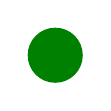
\begin{tikzpicture}[scale=0.7, baseline=0.9mm]%
          \definecolor{slopegreen}{rgb}{0.0, 0.5, 0.0}%
          \fill[slopegreen] (0.5,0.5) circle (0.5);%
        \end{tikzpicture}%
      }%
      {2}{
        
\begin{tikzpicture}[scale=0.7, baseline=0.9mm]%
          \definecolor{slopeblue}{rgb}{0.0, 0.44, 1.00}
          \fill[slopeblue] (0,0) rectangle (1,1);%
        \end{tikzpicture}%
      }%
      {3}{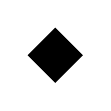
\begin{tikzpicture}[scale=0.7, baseline=0.9mm]\fill (0,0.5)--(0.5, 0)--(1,0.5)--(0.5,1)--cycle; \end{tikzpicture}}%
      {4}{
\begin{tikzpicture}[scale=0.7, baseline=0.9mm]\fill (0.25,0)--(0,0.5)--(0.25,1)--(0.5,0.5)--cycle; \fill (0.75,0)--(0.5,0.5)--(0.75,1)--(1,0.5)--cycle;\end{tikzpicture}}%
      % you can add more cases here as desired
  }[\PackageError{difficulty}{Undefined difficulty level: #1}{}]%
}%
\newcommand{\rating}[2]{\difficulty{#1}\\\score{#2}\\}


\begin{document}
  A polyform counting problem from Alec Jones: let $a_k(n)$ count the number of polyabolos with $n$ faces
  and $k$ exposed edges.
  \begin{figure}[!h]
    \centering
    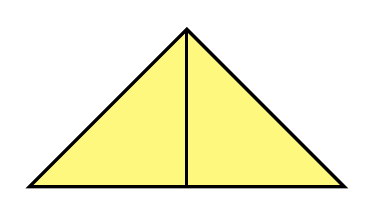
\begin{tikzpicture}[scale=2]
      \draw[very thick, fill={yellow}, fill opacity=0.5] (0,0)--(2,0)--(1,1)--cycle;
      \draw[very thick] (1,1)--(1,0);
    \end{tikzpicture}\hspace{1cm}
    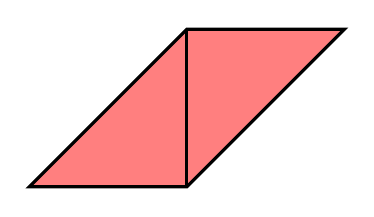
\begin{tikzpicture}[scale=2]
      \draw[very thick, fill={red}, fill opacity=0.5] (0,0)--(1,0)--(2,1)--(1,1)--cycle;
      \draw[very thick] (1,1)--(1,0);
    \end{tikzpicture}
    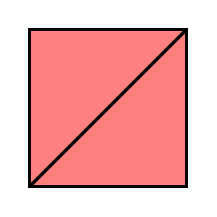
\begin{tikzpicture}[scale=2]
      \draw[very thick, fill={red}, fill opacity=0.5] (0,0)--(1,0)--(1,1)--(0,1)--cycle;
      \draw[very thick] (0,0)--(1,1);
    \end{tikzpicture}\hspace{1cm}
    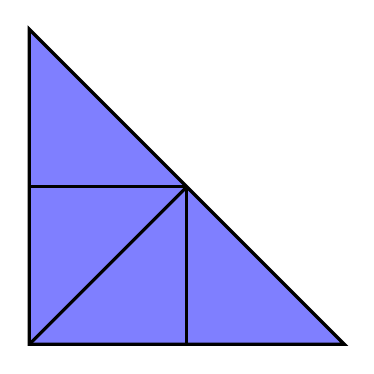
\begin{tikzpicture}[scale=2]
      \draw[very thick, fill={blue}, fill opacity=0.5] (0,0)--(2,0)--(0,2)--cycle;
      \draw[very thick] (0,1)--(1,1);
      \draw[very thick] (0,0)--(1,1);
      \draw[very thick] (1,0)--(1,1);
    \end{tikzpicture}
    \caption{
      An example in yellow showing that $a_3(2) \geq 1$,
      two examples in red showing that $a_4(2) \geq 2$, and
      an example in blue showing that $a_3(4) \geq 1$.
    }
  \end{figure}
\begin{question}
  What is the smallest $k$ such that for some fixed $n$, $a_k(n) > 0$?
\end{question}
\begin{related}
  \item What is the largest $k$ such that for some fixed $n$, $a_k(n) > 0$?
  \item What if $\hat{a}_k(n)$ counts polyiamonds instead?
  \item What if concave polygons are excluded?
  \item Is the following function well-defined? \[
    b(k) = \max \{\,a_k(n) : n \in \mathbb{N} \,\}
  \]
  \item Is the following function interesting? \[
    c(n) = \max \{\,a_k(n) : k \in \mathbb{N} \,\}
  \]
\end{related}
\begin{references}
  \item \url{https://en.wikipedia.org/wiki/Polyiamond}
  \item \url{https://en.wikipedia.org/wiki/Polyabolo}
\end{references}

\end{document}
